% -*- root: ../presentation.tex -*-
\section{Model}

%==============================================================================
\subsection{Reservoir properties}
\begin{frame}
    \frametitle{Reservoir Properties}
    \begin{itemize}
        \item Black Oil fluid model used.
        \item The initial fluids present are water, oil and solution gas.
        \begin{itemize}
            \item The reservoir is undersaturated $\rightarrow$ no free gas.
        \end{itemize}
        \item Note that the porosity in the paper is given as
        \begin{equation}
            \phi = \phi^* [1 + c_\phi (p_o - p^*)],
        \end{equation}
        which corresponds to values in the range $[0.20000,0.20004]$. However, this is approximated to $0.2$.
    \end{itemize}
\end{frame}

\subsection{Original Grid Model}
\begin{frame}
    \frametitle{Original Grid Model}
    \begin{itemize}
        \item $9 \times 9 \times 6$ grid.
        \item One producer and one injector.
        \item Constant $\Delta x$.
        \item Variable $\Delta y$ and $\Delta z$.
        \item Smaller blocks around the producer.
    \end{itemize}
\end{frame}
%==============================================================================



%==============================================================================
\begin{frame}
    \frametitle{Original Grid Model - Top view}
    \footnotesize
    \vspace{-1.5em}
    \begin{center}
        % -*- root: ../../eclipse-data.tex -*-

\begin{tikzpicture}
  \draw[color=lightgray,fill=lightgray] (0,4.39) rectangle (9,4.61); % Injector
  \draw[color=lightgray,fill=gray] (1,4.40) rectangle (8,4.60); % Producer

  \draw[] (0,0) to (0,9) to (9,9) to (9,0) to (0,0);
  \foreach \x in {1,2,...,9} {
    \draw[] (\x,9) to (\x, 0);
    \node[anchor=south] at ($ (\x,9) - (.5,0) $) {\x};
  }

  \draw[] (0,2) to (9,2);
  \draw[] (0,7) to (9,7);

  \draw[] (0,3.5) to (9,3.5);
  \draw[] (0,5.5) to (9,5.5);

  \draw[] (0,4) to (9,4);
  \draw[] (0,5) to (9,5);

  \draw[] (0,4.35) to (9,4.35);
  \draw[] (0,4.65) to (9,4.65);

  \node[anchor=east] at (0,1,00) {\footnotesize 9};
  \node[anchor=east] at (0,2.75) {\footnotesize 8};
  \node[anchor=east] at (0,3.75) {\footnotesize 7};
  \node[anchor=east] at (0,4.15) {\footnotesize 6};
  \node[anchor=east] at (0,4.50) {\footnotesize 5};
  \node[anchor=east] at (0,4.85) {\footnotesize 4};
  \node[anchor=east] at (0,5.25) {\footnotesize 3};
  \node[anchor=east] at (0,6.25) {\footnotesize 2};
  \node[anchor=east] at (0,8.00) {\footnotesize 1};

  \node[anchor=west] at (9,1,00) {\footnotesize 620 ft};
  \node[anchor=west] at (9,2.75) {\footnotesize 400 ft};
  \node[anchor=west] at (9,3.75) {\footnotesize 200 ft};
  \node[anchor=west] at (9,4.15) {\footnotesize 100 ft};
  \node[anchor=west] at (9,4.50) {\footnotesize 60  ft};
  \node[anchor=west] at (9,4.85) {\footnotesize 100 ft};
  \node[anchor=west] at (9,5.25) {\footnotesize 200 ft};
  \node[anchor=west] at (9,6.25) {\footnotesize 400 ft};
  \node[anchor=west] at (9,8.00) {\footnotesize 620 ft};

  \node[anchor=south west] at (9,9) {\footnotesize $\Delta y$};
  \node[anchor=north] at (4.5,0) {\footnotesize $\Delta x = 300 \mathrm{ft} = \mathrm{constant}$};

  \draw[color=lightgray,fill=lightgray] (0,-1.39) rectangle (2,-1.61); % Injector
  \node[anchor=south west] at (2,-1.41) {Producing well (\emph{b} cases)};
  \draw[color=gray,fill=gray] (0,-1.00) rectangle (2,-1.20); % Producer
  \node[anchor=south west] at (2,-1.81) {Injection well};



\end{tikzpicture}

    \end{center}
\end{frame}
%==============================================================================


%==============================================================================
\begin{frame}
    \frametitle{Original Grid Model - Side view}
    \begin{center}
        % -*- root: ../../plots.tex -*-
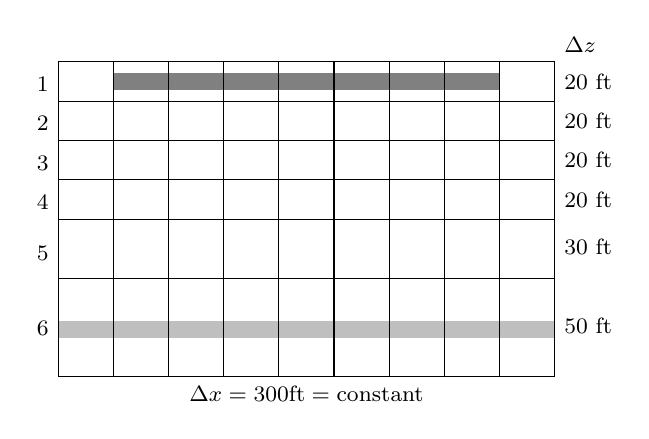
\begin{tikzpicture}[xscale=0.7]
    \draw[color=lightgray,fill=lightgray] (0,.50) rectangle (9,.70);
    \draw[color=gray,fill=gray] (1,3.65) rectangle (8,3.85);

    \foreach \x in {0,1,...,9} {
        \draw[] (\x,0) to (\x,4);
    }
    \draw[] (0,0.00) to (9,0.00);
    \draw[] (0,1.25) to (9,1.25);
    \draw[] (0,2.00) to (9,2.00);
    \draw[] (0,2.50) to (9,2.50);
    \draw[] (0,3.00) to (9,3.00);
    \draw[] (0,3.50) to (9,3.50);
    \draw[] (0,4.00) to (9,4.00);

    \node[anchor=south east] at (0,3.5) {\footnotesize1};
    \node[anchor=south east] at (0,3.0) {\footnotesize2};
    \node[anchor=south east] at (0,2.5) {\footnotesize3};
    \node[anchor=south east] at (0,2.0) {\footnotesize4};
    \node[anchor=south east] at (0,1.35) {\footnotesize 5};
    \node[anchor=south east] at (0,0.40) {\footnotesize 6};

    \node[anchor=south west] at (9,4) {\footnotesize $\Delta z$};
    \node[anchor=west] at (9,3.75) {\footnotesize 20 ft};
    \node[anchor=west] at (9,3.25) {\footnotesize 20 ft};
    \node[anchor=west] at (9,2.75) {\footnotesize 20 ft};
    \node[anchor=west] at (9,2.25) {\footnotesize 20 ft};
    \node[anchor=west] at (9,1.65) {\footnotesize 30 ft};
    \node[anchor=west] at (9,0.65) {\footnotesize 50 ft};
    \node[anchor=north] at (4.5,0) {\footnotesize $\Delta x = 300 \mathrm{ft} = \mathrm{constant}$};
\end{tikzpicture}

    \end{center}
\end{frame}
%==============================================================================


%==============================================================================
\begin{frame}
    \frametitle{Original Grid Model - 3D}
    \begin{center}
        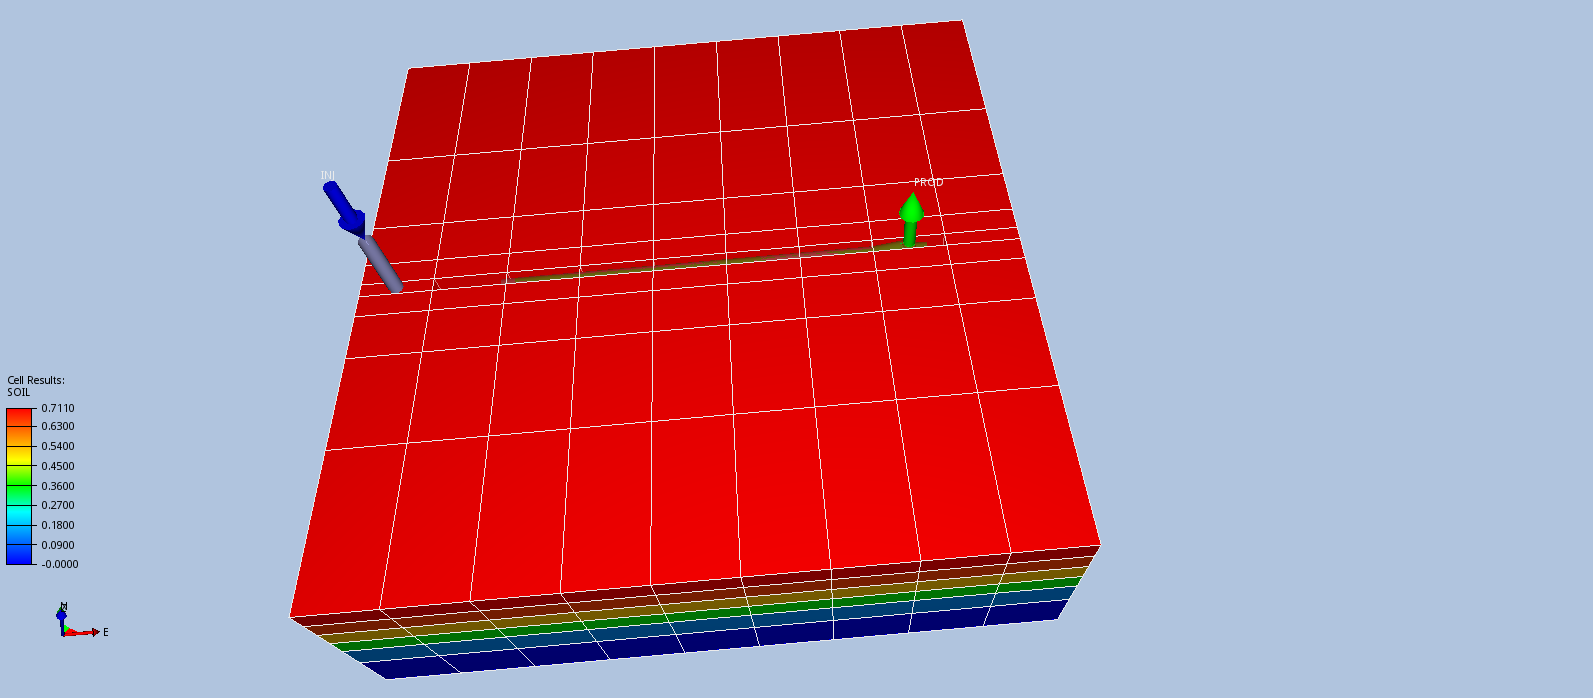
\includegraphics[width=\textwidth]{figures/resinsight/1b-start.png}
    \end{center}
\end{frame}
%==============================================================================


%==============================================================================
\begin{frame}
    \frametitle{Original Grid Model - Wells}
    \begin{itemize}
        \item The model has two wells:
            \begin{itemize}
                \item Producer in top layer.
                \item Injector in bottom layer.
            \end{itemize}
        \item There are two variations on the model:
        \begin{itemize}
             \item short producing well with $L=900$ ft, spanning blocks $(I,5,1), I=6,7,8$.
             \item long producing well with $L=2100$ ft, spanning blocks $(I,5,1), I=2,3,\dots,8$.
        \end{itemize}
        \item In both cases the injector spans blocks $(I,5,6),I=1,2,\dots,9$.
    \end{itemize}
\end{frame}
%==============================================================================


%==============================================================================
\subsection{Refined Grid Model}
\begin{frame}
    \frametitle{Refined Grid Model}
    \begin{itemize}
        \item The ECL100 section of the paper describes how they performed the simulation. It includes a Local Grid Refinement (LGR) around the producing well.
        \begin{itemize}
            \item The top layer is split into three new layers with $\Delta z = 8ft, 4ft, 8ft$. The middle layer contains the well.
            \item The original center row is split into three new rows with $\Delta y = 24ft, 12ft, 24ft$.
            \item Two blocks at each end of the producing well were refined into four new blocks with equal $\Delta x$ values.
        \end{itemize}
        \item This results in \emph{two} different $13 \times 11 \times 8$ grids because the grid is refined differently for the two different well placements.
        \item In the paper this is implemented using the LGR extension. I decided to refine the global grid.
    \end{itemize}
\end{frame}
%==============================================================================


%==============================================================================
\begin{frame}
    \frametitle{Refined Grid Model - Top view (Long well)}
    \begin{center}
        % -*- root: ../eclipse-data.tex -*-

% In Cases 4a and 4b the grid was not refined.Cases 1 to 3 the grid is refined as described below.

% In The aspect ratio of the well blocks in the yz- direction is approximately unity when transformed to an isotropic system, so a refinement that kept this aspect ratio was applied. The refinement was applied to the box of gridblocks consisting of the row of blocks containing the production well plus an extra block on either end. This box was refined as follows: 

% z-direction: 3 layers with Dz = 8 ft, 4 ft, 8 ft 

% y-direction: 3 rows with Dy =24 ft, 12 ft, 24 ft 

% x-direction: 2 blocks at each end of the refinement box were refined into 4, with equal Dx values. The other blocks were not refmed in the x-direction. 

% The refined blocks containing the production well thus had dimensions: 
%    Dx =300 ft and 150 ft; 
%    Dy = 12 ft; 
%    Dz = 4 ft.

% Interpretation: 
%   For long wells: 
%     Row 5, columns 1 and 9, topmost layer.
%     Row five is split into 3 new rows, with thickness 24ft, 12ft, 24ft
%     Column 1,2 and 8,9 is each split into two new blocks, each 150 ft. long
%     Topmost layer is split into three layers, with thickness 8 ft, 4 ft, 8 ft
%
%   Same for short wells, but split blocks 5,6 and 8,9 

% New dimensions: 13x11x8
%    


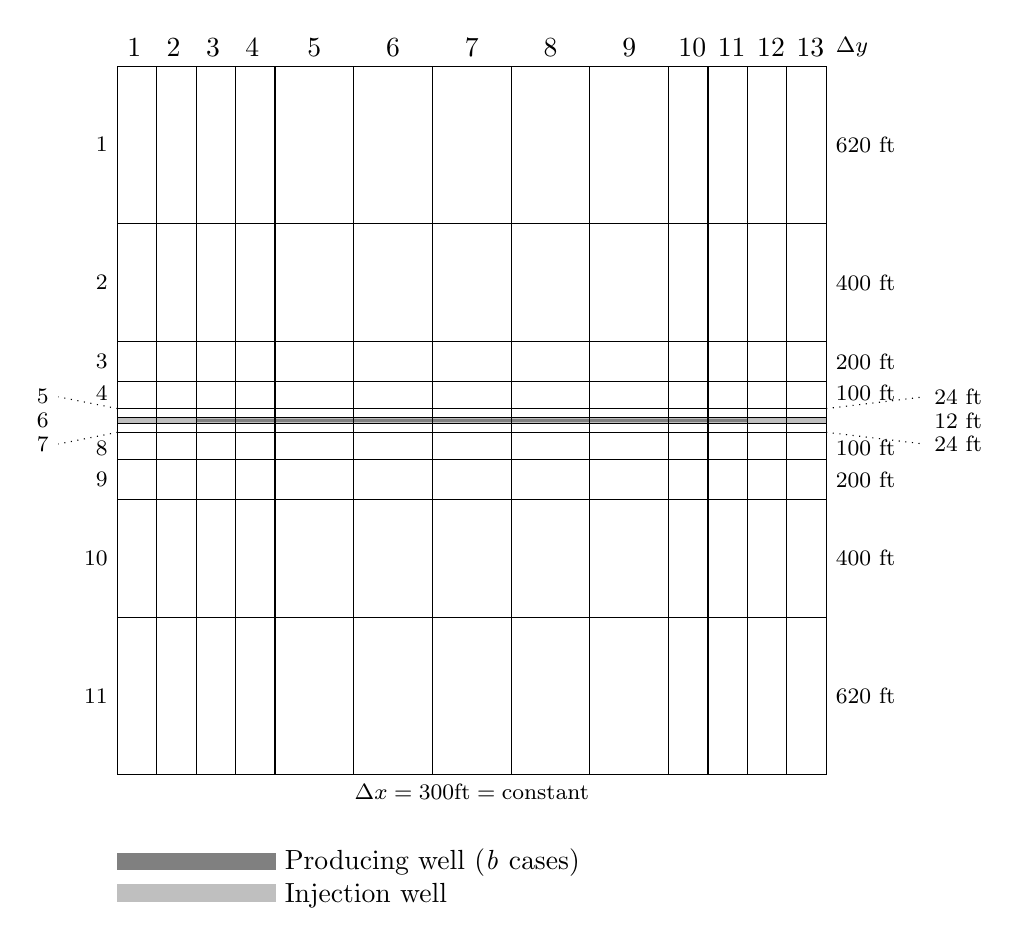
\begin{tikzpicture}
% WELLS =======================================================================
  \draw[color=lightgray,fill=lightgray] (0,4.46) rectangle (9,4.54); % Injector
  \draw[color=lightgray,fill=gray] (1,4.47) rectangle (8,4.53); % Producer

% VERTIVAL LINES ==============================================================
  \draw[] (0,0) to (0,9) to (9,9) to (9,0) to (0,0);
  \foreach \x in {0.5,1,1.5,2,3,4,5,6,7,7.5,8,8.5,9} {
    \draw[] (\x,9) to (\x, 0);
  }

% X-DIRECTION NUMBERING =======================================================
  \node[anchor=south west] at (0.0,9) {1};
  \node[anchor=south west] at (0.5,9) {2};
  \node[anchor=south west] at (1.0,9) {3};
  \node[anchor=south west] at (1.5,9) {4};
  \node[anchor=south     ] at (2.5,9) {5};
  \node[anchor=south     ] at (3.5,9) {6};
  \node[anchor=south     ] at (4.5,9) {7};
  \node[anchor=south     ] at (5.5,9) {8};
  \node[anchor=south     ] at (6.5,9) {9};
  \node[anchor=south west] at (7.0,9) {10};
  \node[anchor=south west] at (7.5,9) {11};
  \node[anchor=south west] at (8.0,9) {12};
  \node[anchor=south west] at (8.5,9) {13};

% HORIZONTAL LINES ============================================================
  \draw[] (0,7) to (9,7); % 1
  \draw[] (0,5.5) to (9,5.5); % 2
  \draw[] (0,5) to (9,5); % 3
  \draw[] (0,4.65) to (9,4.65); % 4
  \draw[] (0,4.54) to (9,4.54); % 6
  \draw[] (0,4.46) to (9,4.46); % 7
  \draw[] (0,4.35) to (9,4.35); % 8
  \draw[] (0,4) to (9,4); % 9
  \draw[] (0,3.5) to (9,3.5); % 10
  \draw[] (0,2) to (9,2); % 11



% Y-DIRECTION NUMBERING
  \node[anchor=east] at (0,1,00) {\footnotesize 11};
  \node[anchor=east] at (0,2.75) {\footnotesize 10};
  \node[anchor=east] at (0,3.75) {\footnotesize 9};
  \node[anchor=east] at (0,4.15) {\footnotesize 8};
  \node[anchor=east] at (-.75,4.20) {\footnotesize 7};
  \node[anchor=east] at (-.75,4.50) {\footnotesize 6};
  \node[anchor=east] at (-.75,4.80) {\footnotesize 5};
  \node[anchor=east] at (0,4.85) {\footnotesize 4};
  \node[anchor=east] at (0,5.25) {\footnotesize 3};
  \node[anchor=east] at (0,6.25) {\footnotesize 2};
  \node[anchor=east] at (0,8.00) {\footnotesize 1};

  \draw[dotted] (0,4.65) to (-.75,4.80);
  \draw[dotted] (0,4.35) to (-.75,4.20);
  

% Y-DIRECTION LENGTHS
  \node[anchor=south west] at (9,9) {\footnotesize $\Delta y$};
  \node[anchor=west] at (9,1,00) {\footnotesize 620 ft};
  \node[anchor=west] at (9,2.75) {\footnotesize 400 ft};
  \node[anchor=west] at (9,3.75) {\footnotesize 200 ft};
  \node[anchor=west] at (9,4.15) {\footnotesize 100 ft};
%  \node[anchor=west] at (9,4.50) {\footnotesize 60  ft};
  \node[anchor=west] at (9,4.85) {\footnotesize 100 ft};
  \node[anchor=west] at (9,5.25) {\footnotesize 200 ft};
  \node[anchor=west] at (9,6.25) {\footnotesize 400 ft};
  \node[anchor=west] at (9,8.00) {\footnotesize 620 ft};

  \draw[dotted] (9,4.65) to (10.25,4.80);
  \draw[dotted] (9,4.35) to (10.25,4.20);
  \node[anchor=west] at (10.25,4.80) {\footnotesize 24 ft};
  \node[anchor=west] at (10.25,4.50) {\footnotesize 12 ft};
  \node[anchor=west] at (10.25,4.20) {\footnotesize 24 ft};

  \node[anchor=north] at (4.5,0) {\footnotesize $\Delta x = 300 \mathrm{ft} = \mathrm{constant}$};

% LEGEND ======================================================================
  \draw[color=lightgray,fill=lightgray] (0,-1.39) rectangle (2,-1.61); % Injector
  \node[anchor=south west] at (2,-1.41) {Producing well (\emph{b} cases)};
  \draw[color=gray,fill=gray] (0,-1.00) rectangle (2,-1.20); % Producer
  \node[anchor=south west] at (2,-1.81) {Injection well};



\end{tikzpicture}

    \end{center}
\end{frame}
%==============================================================================


%==============================================================================
\begin{frame}
    \frametitle{Refined Grid Model - Side view (Long well)}
    \begin{center}
        % -*- root: ../plots.tex -*-
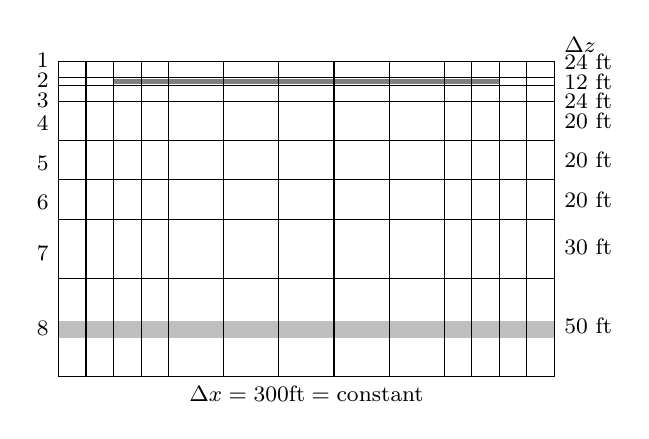
\begin{tikzpicture}[xscale=0.7]
    \draw[color=lightgray,fill=lightgray] (0,.50) rectangle (9,.70);
    \draw[color=gray,fill=gray] (1,3.72) rectangle (8,3.78);

    \foreach \x in {0,.5,1,1.5,2,3,4,5,6,7,7.5,8,8.5,9} {
        \draw[] (\x,0) to (\x,4);
    }
    \draw[] (0,0.00) to (9,0.00);
    \draw[] (0,1.25) to (9,1.25);
    \draw[] (0,2.00) to (9,2.00);
    \draw[] (0,2.50) to (9,2.50);
    \draw[] (0,3.00) to (9,3.00);
    \draw[] (0,3.50) to (9,3.50);
    \draw[] (0,3.70) to (9,3.70);
    \draw[] (0,3.80) to (9,3.80);
    \draw[] (0,4.00) to (9,4.00);

    \node[anchor=south east] at (0,3.80) {\footnotesize 1};
    \node[anchor=south east] at (0,3.55) {\footnotesize 2};
    \node[anchor=south east] at (0,3.30) {\footnotesize 3};
    \node[anchor=south east] at (0,3.0) {\footnotesize 4};
    \node[anchor=south east] at (0,2.5) {\footnotesize 5};
    \node[anchor=south east] at (0,2.0) {\footnotesize 6};
    \node[anchor=south east] at (0,1.35) {\footnotesize 7};
    \node[anchor=south east] at (0,0.40) {\footnotesize 8};

    \node[anchor=south west] at (9,4) {\footnotesize $\Delta z$};
    \node[anchor=west] at (9,4.0) {\footnotesize 24 ft};
    \node[anchor=west] at (9,3.75) {\footnotesize 12 ft};
    \node[anchor=west] at (9,3.50) {\footnotesize 24 ft};
    \node[anchor=west] at (9,3.25) {\footnotesize 20 ft};
    \node[anchor=west] at (9,2.75) {\footnotesize 20 ft};
    \node[anchor=west] at (9,2.25) {\footnotesize 20 ft};
    \node[anchor=west] at (9,1.65) {\footnotesize 30 ft};
    \node[anchor=west] at (9,0.65) {\footnotesize 50 ft};
    \node[anchor=north] at (4.5,0) {\footnotesize $\Delta x = 300 \mathrm{ft} = \mathrm{constant}$};
\end{tikzpicture}

    \end{center}
\end{frame}
%==============================================================================

%==============================================================================
\begin{frame}
    \frametitle{Refined Grid Model - 3D}
    \begin{center}
        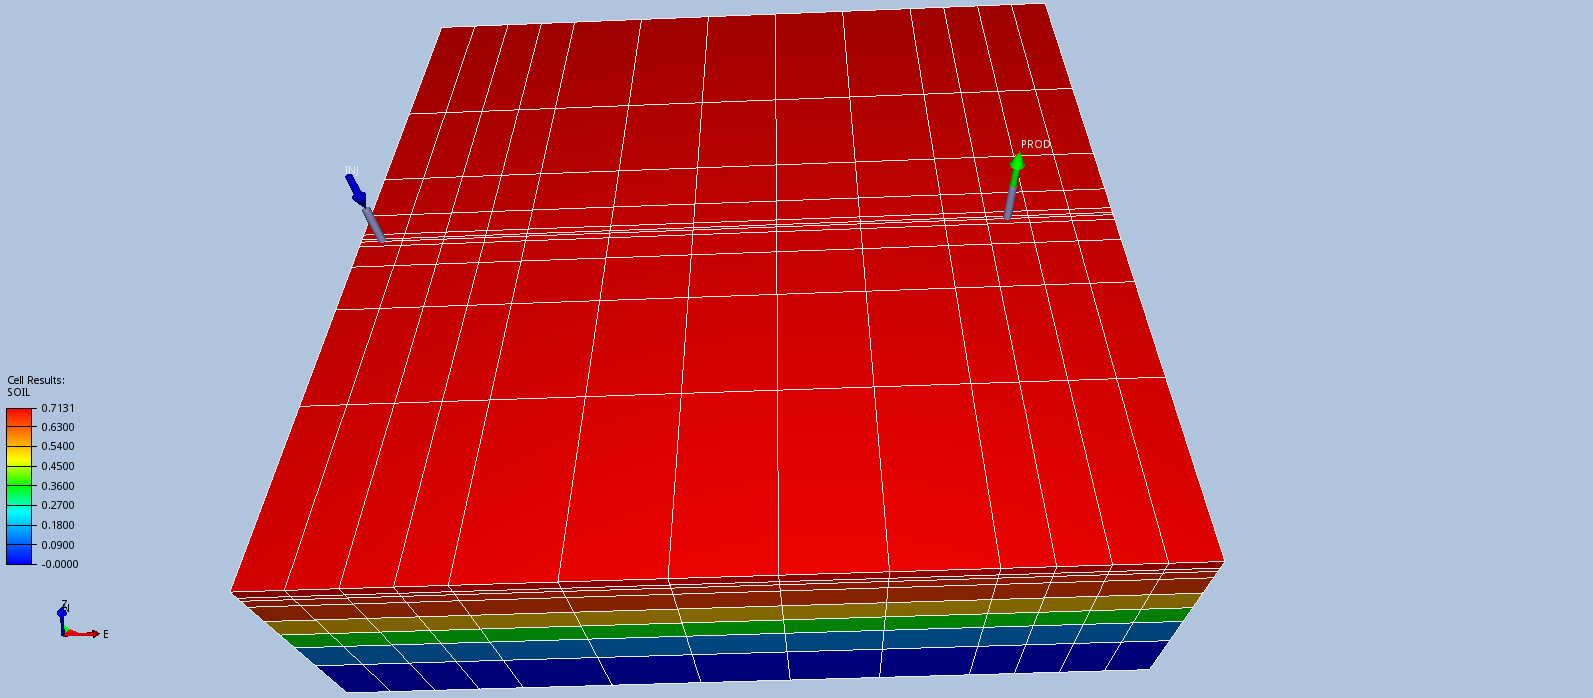
\includegraphics[width=\textwidth]{figures/resinsight/1b-refined-end.png}
    \end{center}
\end{frame}
%==============================================================================


%==============================================================================
\begin{frame}
    \frametitle{Refined Grid Model: Wells}
    \begin{itemize}
        \item Still two wells:
        \begin{itemize}
            \item Producer in second layer from the top.
            \item Injector in bottom layer.
        \end{itemize}
        \item Still two variations on the producer:
        \begin{itemize}
            \item short well with length $L=900$ ft, spanning blocks $(I,6,2), I=7,8,...,11$.
            \item long well with length $L=2100$ ft, spanning blocks $(I,6,2), I=3,4,...,11$.
        \end{itemize}
        \item In both cases the injector spans $(I,6,2), I=1,2,...,13$.
    \end{itemize}
\end{frame}
%==============================================================================